\chapter{Improving the IEBT algorithm} \label{IEBT}
This is the second part of my work, where I will try to find and argue for different improvements for the implementation of the algorithm for incremental enumeration of Bitriagles (IEBT).
This implementation developed by Juan Pablo uses the Dynamic Pipeline library with which I have been working.
The entire first part of my work has been necessary to fully understand the operation of both the dynamic pipeline paradigm itself and the operation of the Haskell library.

\section{Introduction}
A brief introduction to understand the basic concepts is provided here.
For a more detailed explanation, refer to Royo-Sales et al. \cite[][See chapter 6]{royo_sales_algorithm_2021} \\
The IEBT algorithm involves finding bitriangles in a bipartite graph.
\begin{figure}[H]
  \centering
  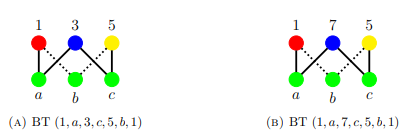
\includegraphics[width=1\textwidth]{JP1.png}
  \caption[{[IEBT] BiTriangle}]{Bitriangle structure, taken from \cite{royo_sales_algorithm_2021}}
  \label{fig:JP1}
\end{figure}
To achieve this, it groups vertices into different structures until it reaches a structure that forms many bitriangles. \\
The process is as follows: initially, all the edges of the graph are processed, and the generator creates a filter for each edge it receives, initializing it with that edge.
The filters process the edges and check the vertices to find a match with their parameter.
If a match is found, it consumes the edge and adds it to its state, thus forming the Aggregated Wedges.
\begin{figure}[H]
  \centering
  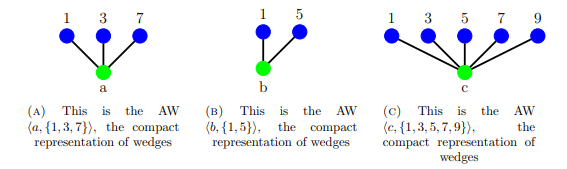
\includegraphics[width=1\textwidth]{JP2.png}
  \caption[{[IEBT] Aggregated Wedges}]{Aggregated Wedges strucute, taken from \cite{royo_sales_algorithm_2021}}
  \label{fig:JP2}
\end{figure}
Once all the edges have been processed, the filters send the AWs generated by the pipeline so that they can be combined to form the Aggregated Double-Wedges.

\begin{figure}[H]
  \centering
  \includegraphics[width=1\textwidth]{JP3.png}
  \caption[{[IEBT] Aggregated Doble Wedges}]{Aggregated Doble Wedges structure, taken from \cite{royo_sales_algorithm_2021}}
  \label{fig:JP3}
\end{figure}

Once the filters have these structures, queries can be sent through the pipeline to obtain the bitriangles.
\section{Improving structures}
The first topic I wanted to address was the data types used to store the different sets.
The algorithm needs to store different vertex structures for later matching.
These are the different definitions found in the code:

\begin{figure}[H]
    %\centering
    \begin{tabular}{c}
        \begin{lstlisting}[escapeinside={(*}{*)}]
type LowerVertex = Int
type UpperVertex = Int
type Edge = (UpperVertex, LowerVertex)

data Command = ByVertex IntSet
            | ByEdge (Set Edge)
            | Count
            | AllBT
            | NoCommand
            | End
        deriving (Show, Read)

data W = W
  { _wLowerVertex :: LowerVertex
  , _wWedges      :: IntSet
  }
  deriving Show

data Triplet = Triplet Int Int Int
data Pair = Pair Int Int

type UT = (IntSet, IntSet, IntSet)

data DW = DW
  { _dwLower :: Pair
  , _dwUpper :: UT
  }

newtype DWTT = DWTT [DW]
  deriving newtype (Semigroup, Monoid)

data BT = BT
  { _btLower :: Triplet
  , _btUpper :: UT
  }

newtype BTTT = BTTT [BT]
  deriving newtype (Semigroup, Monoid)

data BTResult = RBT Q (Int, Int, Int, Int, Int, Int, Int)
              | RC  Q Int

data FilterState = Adj W
                 | DoubleWedges DWTT
                 | BiTriangles BTTT
        \end{lstlisting}
    \end{tabular}
    \caption[{[IEBT] Type and data definitions}]{Type and data definitions of IEBT implementation}
    \label{fig:HC40}
\end{figure}


We can see how it represents vertices with integers Int and edges as tuples of integers (Int, Int).
The most important thing to analyze are the set representations, as their impact on the performance of the algorithm is crucial.
It uses the IntSet structure to represent sets of vertices and also a tuple of 3 IntSets (IntSet, IntSet, IntSet) to represent the set of upper vertex of the Aggregated Doble Wedge and Aggregated Bitriangles. \cite[][Page52]{royo_sales_algorithm_2021}
Also taking into account the use of lists to represent the set of Aggregated Double Wedges and Aggregated Bitriangles. \\

We will be analizing structure by structure trying to find if the structure used is the most efficient.
\subsection{Set of vertices representation}
The IntSet structure belongs to the Haskell IntSet library \cite{noauthor_dataintset_nodate}, which represents an ordered set of Ints.
This structure is very efficient because it takes advantage of the range limit of Ints to limit many operations to a cost of O(min(n,W)), where n is the number of elements and W is the number of bits in the Int representation (32 or 64).
Additionally, this structure is based on big-endian patricia trees, which have very good performance for set intersection and union operations.

\subsubsection*{Wedges representation}
If we review the first structure that use IntSet, we can see that filters can have three types of states, one of which is the Wedge, which uses this structure.
To understand how this structure is used (and therefore whether or not it can be improved), we need to know what computations are performed with it.
Observing the code, we can see that only two of the four actors that each filter has deal with W: actor1 and actor2.\\
On the part of actor1, for each input edge, a condition is checked and if it is affirmative, a vertex is attached to the IntSet set.
Therefore, in the worst case, insertions will have to be made and each insertion has a cost of O(n,W), and assuming a sufficiently large n, we are left with O(W) = O(1). \\
On the other hand, actor2 performs difference and intersection operations with the IntSets.
These operations with this library have a linear cost with respect to the size of the sets O(n + m). \\

Looking at these costs, we can conclude that a very efficient structure seems to be used.
We could also use a Hash-type structure, such as a HashSet, to improve the performance of insertions.
Reviewing the Haskell libraries, we find the HashSet structure.
Despite being useful, the documentation itself warns us that for Int sets, the IntSet library is more efficient.
Therefore, for Wedges, IntSets are the best structure.

\subsubsection*{Doble Wedges and Agregated Bitriangles representation}
Next, we should focus on the definition of the UT type, which is formed by a tuple of 3 IntSets.
If we review the entire code for functions that use it, we find a similar scenario to the previous one.
In general, insertion operations are performed on the sets, and the choice of IntSet is correct. \\

On the other hand, the other important operation that is performed is to check if a vertex belongs to any of the 3 sets.
To do this, it checks each of the 3 sets, so it might be possible to optimize this process a bit.
Despite this, the best option that could be done is to try to join the 3 sets so that you only have to search in a larger one, asymptotically reducing the cost by 3.
The problem is that we would have to find another way to represent the 3 sets, such as with indexes using a dictionary.
For this reason, I have considered that the cost of carrying this structure and other operations that are done on it increases greatly for the improvement we obtain, so I do not see any possible improvement in this regard. \\

Therefore, the choice of this structure is the correct one to represent the UTs.

\subsection{Set of edges representation}
The next thing to observe is the representation of edge sets.
As such, the entire algorithm does not store any edge sets, as it plays with the structure of the different types to infer the edges.
There is only one thing for which edges are used: the final Queries. \\

At this stage, a set of edges can be passed to find bitriangles that contain it, and for this, it uses the Set to store them.
In this case, the only operation that is done is to check whether an edge is inside or not.
Therefore, I have determined that a possible improvement could be to change the Set, which has a search cost of O(log n), to one that has better performance, such as the HashSet.
The HashSet has a cost, in the general case, of constant O(1). \\

Therefore, I have changed the Set structure to HashSet to look for a performance improvement.
At the end of the work \ref{experiments}, an experimental test will be carried out to verify whether there is an improvement or not.

\section{Chapter Summary}
In this chapter, we have been analyzing the implementation of the IEBT algorithm to try to find an improvement. \\
Despite the fact that the beginning of this work arose with the belief that it could be improved, I have not been able to find a possible significant improvement for the implementation of the IEBT algorithm.
